\chapter{Optimierung - Mathematische Grundlagen und Methoden}\label{cha:Optimierung}
In diesem Kapitel werden die notwendigen mathematischen Grundlagen beschrieben, die zur Formulierung eines \gls{OP} und zur Lösung mithilfe der Variationsrechnung notwendig sind. Dazu wird zunächst der Unterschied zwischen \textit{statischer} und \textit{dynamischer} Optimierung erläutert und anschließend mit der \textit{Variationsrechnung} eine Lösungsmethode eingeführt, mit der sich ein dynamisches \gls{OP} in ein System nichtlinearer \gls{DGL} 1. Ordnung überführen lässt, dessen Lösung entweder analytisch oder numerisch bestimmt werden kann. Danach werden zusätzliche Methoden erläutert, mit deren Hilfe sich ein komplexes \gls{OP} in mehrere miteinander verknüpfte Optimierungsaufgaben unterteilen lässt, deren Lösungen vergleichsweise einfach bestimmt werden können. Abschließend werden einige Lösungsverfahren zur numerischen Lösung dynamischer \gls{OP} vorgestellt und diskutiert. 
\section{Statische Optimierung}\label{sec:statischeOpt}
Die allgemeine Standardformulierung eines statischen \gls{OP} lautet \cite{KnutGraichen.2012}:
\begin{align}
	\min_{\ve{x}\in\mathbb{R}^n} \quad &\fofx \label{eq:J_statisch}\\
	\textrm{u.B.v.} \quad&\mathbf{g}(\ve{x}) = 0 \label{eq:GNB_statisch}\\
	&\mathbf{h}(\ve{x}) \leq 0 \label{eq:UNB_statisch}
\end{align}
Die Funktion \fofx\,wird dabei als Kosten- oder Gütefunktion bezeichnet und bezüglich der Optimierungsvariablen $\ve{x}$ unter Berücksichtigung der Nebenbedingungen $\mathbf{g}$ und $\mathbf{h}$ minimiert. Bei der statischen Optimierung sind die Variablen $\ve{x}$ Elemente des Euklidischen Raums \cite{KnutGraichen.2012}. Für die \gls{GNB} $\mathbf{g}(\ve{x})$ und die \gls{UNB} $\mathbf{h}(\ve{x})$ gilt $\mathbf{g}\in\mathbb{R}^p$ bzw. $\mathbf{h}\in\mathbb{R}^q$, wobei $p<n$ sein muss, da sich die Optimierungsvariablen $\ve{x}$ ansonsten bei $p=n$ unabhängigen Gleichungen direkt aus $\mathbf{g}(\ve{x})$ bestimmen lassen \cite{Papageorgiou.2012}. Für die Anzahl der \gls{UNB} hingegen gibt es keine maximal zulässige Anzahl \cite{Papageorgiou.2012}.
\section{Dynamische Optimierung}\label{sec:dynamischeOpt}
Im Unterschied zur statischen Optimierung sind die Optimierungsvariablen bei der dynamischen Optimierung selbst Funktionen einer unabhängigen Variable, welche in den meisten Fällen der Zeit $t$ entspricht \cite{KnutGraichen.2012}. Das bedeutet, es werden die optimalen Zeitverläufe der Optimierungsvariablen gesucht. Aufgrund dessen wird die Funktion \fofx\,zum Kosten- oder Gütefunktional \J, welches bei der dynamischen Optimierung minimiert wird. Eine sehr häufige Anwendung der dynamischen Optimierung findet man bei dynamischen Systemen, für die eine optimale Eingangstrajektorie \uoptoft\,gesucht wird \cite{KnutGraichen.2012}. Da es sich bei den Optimierungsvariablen um die Eingangs- bzw. Steuergrößen des Systems handelt, wird auch von einem \textit{Optimalsteuerungsproblem} gesprochen \cite{KnutGraichen.2012}. Gleichzeitig liefert die Lösung des Problems die optimalen Zustandstrajektorien \xoptoft, weshalb die Formulierung eines dynamischen \gls{OP} einen geeigneten Ansatz zur Trajektorienplanung dynamischer Systeme darstellt. 
Die allgemeine Formulierung eines solchen Optimalsteuerungsproblems lautet \cite{KnutGraichen.2012}:
\begin{align}
\min_{\uoft} \quad &J(\xoft,\uoft,t,t_f) = \Vofxoftf + \int_{t_0}^{t_f}l(\xoft,\uoft,t)\dtint{t} \label{eq:J_dyn}\\
\textrm{u.B.v.} \quad& \dxoft = \ve{f}(\xoft,\uoft,t)\,,\qquad \xoftzero = \xzero \label{eq:system_anfang}\\
&\mathbf{g}(\xoftf,t_f) = 0 \label{eq:GNB}\\
&\mathbf{h}(\xoft,\uoft) \leq 0 \label{eq:UNB}
\end{align}
Es gilt $\ve{x}\in\mathbb{R}^n, \ve{u}\in\mathbb{R}^m, \mathbf{g}\in\mathbb{R}^p$ und $\mathbf{h}\in\mathbb{R}^q$. Wie bereits bei der statischen Optimierung stellen die Gleichungen \eqref{eq:GNB} und \eqref{eq:UNB} \gls{GNB} und \gls{UNB} dar, wobei die \gls{UNB} an dieser Stelle lediglich der Vollständigkeit halber in der allgemeinen Form mit angegeben sind. Für die weiteren Betrachtungen - die Anwendung der Variationsrechnung und die Ergebnisse dieser Arbeit - spielen die \gls{UNB} keine Rolle. Es sei allerdings darauf hingewiesen, dass sich auch Optimalsteuerungsprobleme mit \gls{UNB} mithilfe des Ansatzs der Variationsrechnung lösen lassen. Für weitere Informationen zum Umgang mit allgemeinen \gls{UNB} für die Systemzustände und/oder Eingangsgrößen sei auf entsprechende Fachliteratur zum Thema Optimierung verwiesen (siehe \cite{Papageorgiou.2012, Gerdts.2010}). Gleichung \eqref{eq:system_anfang} beschreibt die Systemdynamik mit der Eingangsgröße \uoft\,und die Anfangszustände \xzero\,des Systems, die als Randbedingungen fungieren. Das Gütefunktional in Gleichung \eqref{eq:J_dyn} wird in der dargestellten Form auch als \textit{Bolza-Form} des Gütefunktionals bezeichnet und setzt sich aus zwei Teilen zusammen: Der Integralanteil beschreibt die von der Zeit abhängigen laufenden Kosten und heißt \textit{Lagrange-Form}. Der vor dem Integralanteil stehende Term \Vofxoftf\,gibt die Bewertung des Endzustands (und der Endzeit), also die Endkosten, an. Dieser wird \textit{Mayer-Form} genannt \cite{KnutGraichen.2012}. Für die Lagrange- und Bolza-Form gilt, dass sie sich immer in die Mayer-Form überführen lassen \cite{KnutGraichen.2012} (siehe auch \cite{Gerdts.2010}). Der Endzeitpunkt $t_f$ kann festgelegt sein oder frei. Ist er frei, so muss $t_f$ als zusätzliche Optimierungsvariable bei der Lösung des \gls{OP} berücksichtigt werden \cite{KnutGraichen.2012}. 
\subsection{Variationsrechnung}\label{subsec:Variationsrechnung}
Die Variationsrechnung bietet einen Ansatz, mit dem dynamische \gls{OP}, wie im vorherigen Absatz vorgestellt, gelöst werden können. Dazu werden ausgehend von den optimalen Trajektorien \xoptoft\,und \uoptoft\,und dem optimalen Endzeitpunkt \opt{t_f} (sofern $t_f$ frei und damit Teil der Optimierung ist) Variationen zugelassen, sodass gilt \cite{KnutGraichen.2012}:
\begin{align}
\xoft &= \xoptoft + \epsilon\variation{x}(t) \label{eq:x_var}\\
\dxoft &= \dxoptoft + \epsilon\variation{\dot{x}}(t) \label{eq:dx_var}\\
\uoft &= \uoptoft + \epsilon\variation{u}(t) \label{eq:u_var}\\
t_f &= \opt{t_f} + \epsilon\delta_{t_f}\label{eq:t_var}
\end{align}
Die $\ve{\delta}$-Variablen bezeichnen dabei die Variationen der einzelnen Größen und $\epsilon$ ist der Parameter, mit dem die Variationen Einfluss auf die Trajektorien nehmen, wobei für $\epsilon=0$ offensichtlich $\xoft=\xoptoft$, $\dxoft = \dxoptoft$, $\uoft=\uoptoft$ und $t_f=\opt{t_f}$ gilt. In Abbilung \ref{fig:Variation} ist ein solcher Verlauf einer möglichen optimalen Trajektorie \xoptoft\,und einer zulässigen Variation skizziert. Außerdem sind die Variation des Endzeitpunkts und des Endzustands $\xoftf = \xoptoftfopt+\epsilon(\variation{x}(\opt{t_f})+\dxoptoftfopt\delta_{t_f})$ (falls, \xoftf\,frei ist) dargestellt.
\begin{figure}[h]
\centering
\begin{tikzpicture}[scale=1.5, domain=0:4, samples=200]
\draw[->] (0,0) -- (5,0) node[right] {$t$};
\draw[->] (0,0) -- (0,4) node[above] {$x$};
\draw[color=black,domain=0:4,-*]    plot (\x,{sqrt(\x)});
\draw[color=red,domain=0:4.5,-*]   plot (\x,{sqrt(\x)+0.5*sin(3*\x r)});
\draw [dashed] (3.95,0) node[below] {$\opt{t_f}$} -- (3.95,3);
\draw [dashed] (4.45,0) node[below] {$t_f$} -- (4.45,3);
\draw[-] (4.45,2.5) -- (4.8,2.5);
\draw[-] (3.95,2) -- (4.8,2);
\draw [stealth-stealth] (3.95,0.7) -- (4.45,0.7) node[midway,above] {$\delta_{t_f}$};
\draw [stealth-stealth] (4.7,2) -- (4.7,2.5) node[midway,right] {$\variation{x}(\opt{t_f})+\dxoptoftfopt\delta_{t_f}$};
\draw [-stealth] (2.7,0.7) node[below] {$\xoptoft + \epsilon\variation{x}(t)$} -- (3.3,1.4) ;
\draw [-stealth] (1.3,2) node[above] {\xoptoft} -- (1.5,1.3) ;
\draw [-stealth] (3.2,2.5) node[above] {$\xoptoftfopt$} -- (3.8,2.1) ;
\end{tikzpicture}
\caption{Schematische Darstellung der optimalen Trajektorie \xoptoft\,und eine mögliche, zulässige Variation \xoft.}
\label{fig:Variation}
\end{figure}

Für die Anwendung der Variationsrechnung zur Optimierung dynamischer Systeme wird das folgende Gütefunktional definiert \cite{KnutGraichen.2012}:
\begin{equation}
J(\xoft,\dxoft,\uoft,t,t_f) = \Vofxoftf + \int_{t_0}^{t_f}l(\xoft,\uoft,t) + \lambdaoft^T(\ve{f}(\xoft,\uoft,t) - \dxoft)\dtint{t} \label{eq:J_var_sys}
\end{equation}
Im Vergleich zu \eqref{eq:J_dyn} wurde das Gütefunktional um den Term $\lambdaoft^T(\ve{f}(\xoft,\uoft,t) - \dxoft)$ erweitert, wobei dieser für $\dxoft = \ve{f}(\xoft,\uoft,t)$ zu null wird. Die Variablen $\ve{\lambda}\in\mathbb{R}^n$ stellen dabei die sogenannten \textit{adjungierten Zustände} dar \cite{KnutGraichen.2012}. Werden die Variablen im Gütefunktional nun durch die Gleichungen \eqref{eq:x_var}-\eqref{eq:t_var} ersetzt, hängt das Gütefunktional nur noch von $\epsilon$ ab. Da die Trajektorien \xoft, \dxoft\,und \uoft\,wie bereits gezeigt nur für $\epsilon=0$ den optimalen Verläufen entsprechen können, lautet die notwendige Bedingung für das Verschwinden der Variation des Gütefunktionals $\delta_J$ und damit für ein Minimum 
\begin{equation}
	\delta_J = \frac{\textrm{d}J(\xoptoft+\epsilon\variation{x}(t),\dxoptoft + \epsilon\variation{\dot{x}}(t),\uoptoft + \epsilon\variation{u}(t),\opt{t_f} + \epsilon\delta_{t_f})}{\dtint{\epsilon}}_{|\epsilon=0}=0\,. \label{eq:VariationJ}
\end{equation}
Aus dieser Bedingung lassen sich die notwendigen Optimalitätbedingungen für eine optimale Lösung herleiten. Auf die vollständige Herleitung der Gleichungen wird an dieser Stelle verzichtet und auf weiterführende Literatur verwiesen \cite{KnutGraichen.2012,Papageorgiou.2012,Gerdts.2010}.
\subsubsection{Optimalitätsbedingungen}\label{subsubsec:Optimalitätsbedingungen}
Zunächst wird die \textit{Hamilton-Funktion} als 
\begin{equation}
	H(\xoft,\uoft,\lambdaoft,t) = l(\xoft,\uoft,t) + \lambdaoft^T\ve{f}(\xoft,\uoft,t) \label{eq:Hamilton}
\end{equation}
definiert, mit deren Hilfe die Optimalitätsbedingungen angegeben werden können. Im Folgenden wird auf die explizite Nennung aller Argumente, dort wo diese nicht unbedingt notwendig sind, aus Gründen der Übersichtlichkeit verzichtet. Damit die notwendige Bedingung für ein Minimum \eqref{eq:VariationJ} erfüllt sein kann, müssen die folgenden Optimalitätsbedingungen erfüllt sein \cite{KnutGraichen.2012}.
\begin{align}
	\dx &= \frac{\partial H}{\partial\ve{\lambda}} = \ve{f}(\ve{x},\ve{u},t) \label{eq:Zustandsdgl} \\
	\dlambda &= -\frac{\partial H}{\partial \ve{x}} \label{eq:Adjdgl} \\
	\ve{0} &= \frac{\partial H}{\partial \ve{u}} \label{eq:Steuerungsgleichung} 
\end{align}
Gleichung \eqref{eq:Zustandsdgl} beschreibt die Zustandsdifferentialgleichung, während Gleichung \eqref{eq:Adjdgl} die \gls{DGL} für die adjungierten Zustände $\ve{\lambda}$ beschreibt und daher auch \textit{adjungierte \gls{DGL}} genannt wird \cite{Konigorski.2019}. Die beiden Gleichungen \eqref{eq:Zustandsdgl} und \eqref{eq:Adjdgl} werden auch als \textit{kanonische \gls{DGL}} bezeichnet und bilden gemeinsam mit der Steuerungsgleichung \eqref{eq:Steuerungsgleichung} die sogenannten \textit{Hamiltongleichungen} \cite{Konigorski.2019}. Die kanonischen \gls{DGL} lassen sich zu einer gemeinsamen Systemdynamik 
\begin{equation}
	\dz = \begin{bmatrix}
	\dx \\
	\dlambda
	\end{bmatrix} = 
	\begin{bmatrix}
	\ve{f}(\ve{x},\ve{u},t) \\
	-\frac{\partial H}{\partial \ve{x}}
	\end{bmatrix} \label{eq:Sysdyn_z}
\end{equation}
zusammenfassen.
Die Randbedingungen für das \gls{OP} ergeben sich zu \cite{KnutGraichen.2012}
\begin{align}
\xoftzero &= \xzero \label{eq:Anfangswerte} \\
x_i(t_f) &= x_{f,i}\,, \quad i \in\mathcal{I}_f \label{eq:Endwerte} \\
\lambda_i(t_f) &= \frac{\partial V}{\partial x_i}_{|t=t_f}\,, \quad i \notin \mathcal{I}_f \label{eq:Lambdaend} \\
H(\ve{x},\ve{u},\ve{\lambda},t)_{|t=t_f} &= -\frac{\partial V}{\partial t}_{|t=t_f}\,,\quad \textrm{falls, $t_f$ frei ist.} \label{eq:Transversalitaet}
\end{align}
Die Gleichungen \eqref{eq:Anfangswerte} und \eqref{eq:Endwerte} geben die Randbedingungen für die Anfangs- und Endwerte der Zustände an. $\mathcal{I}_f$ bezeichnet dabei die Menge aller Zustände, die explizit über Endbedingungen vorgegeben sind - eine Vorgabe der Endwerte ist nicht zwingend notwendig. Für solche Zustände, deren Endwert nicht vorgegeben und damit frei ist, gilt Gleichung \eqref{eq:Lambdaend}. Gleichung \eqref{eq:Transversalitaet} gilt nur dann, falls $t_f$ frei und damit eine Optimierungsvariable des Problems ist und gibt so die zusätzliche notwendige Gleichung zur Bestimmung der freien Endzeit an. Die Gleichungen \eqref{eq:Lambdaend} und \eqref{eq:Transversalitaet} werden als \textit{Transversalitätsbedingungen} bezeichnet \cite{KnutGraichen.2012}. 
\subsubsection{Singulärer Fall}\label{subsubsec:Singularität}
In der Regel lässt sich die Eingangsgröße aus der Steuerungsgleichung \eqref{eq:Steuerungsgleichung} durch die Systemzustände und die adjungierten Zustände ausdrücken, wobei dies nicht immer der Fall sein muss \cite{KnutGraichen.2012}. Für \gls{OP}, die ein eingangsaffines System optimieren und in denen $l(\ve{x},\ve{u},t)$ unabhängig von $\ve{u}$ ist, gilt 
\begin{equation}
	\frac{\partial H}{\partial \ve{u}} = \frac{\partial (l(\ve{x},t) + \ve{\lambda}^T(\ve{f}_0(x)+\ve{f}_1(x)\ve{u}))}{\partial \ve{u}} = \ve{\lambda}^T\ve{f}_1(x) = 0 \,. \label{eq:dhduzero}
\end{equation}
Die Darstellung $\ve{f}(\ve{x},\ve{u},t) = \ve{f}_0(x)+\ve{f}_1(x)\ve{u}$ verdeutlicht dabei die Eingangsaffinität des dynamischen Systems. Aus Gleichung \eqref{eq:dhduzero} ist direkt zu erkennen, dass sich die Steuergröße \uoft\,in diesem Fall nicht durch die Zustände ausdrücken lässt, weshalb auch von einem \textit{singulären} Problem gesprochen wird \cite{KnutGraichen.2012}. Der singuläre Fall kann allerdings in der Praxis leicht umgangen werden, indem die Stellgröße mithilfe von hinreichend kleinen Gewichtungen zum Gütefunktional hinzugefügt wird, sodass der Einfluss auf das Optimierungsergebnis vernachlässigbar gering ist, aber trotzdem $\frac{\partial l(\ve{x},\ve{u},t)}{\partial \ve{u}} \neq 0$ gilt \cite{KnutGraichen.2012}.
\subsubsection{Allgemeine Endbedingungen}\label{subsubsec:Allg_Endbedingungen}
Damit neben der Vorgabe einzelner Endzustände auch allgemeine Endbedingungen, wie in Gleichung \eqref{eq:GNB} dargestellt, berücksichtigt werden können, wird das Gütefunktional in Gleichung \eqref{eq:J_var_sys} wie folgt erweitert. Das Funktional zur Betrachtung allgemeiner Endbedingungen lautet
\begin{equation}
J(\ve{x},\dx,\ve{u},t,t_f) = \underbrace{\Vofxoftf + \ve{\nu}^T\mathbf{g}(\xoftf,t_f)}_{\Vofxoftfallgemein} + \int_{t_0}^{t_f}l(\ve{x},\ve{u},t) + \ve{\lambda}^T(\ve{f}(\ve{x},\ve{u},t) - \dx)\dtint{t}\,. \label{eq:J_var_sys_allgemein}
\end{equation}
Über die \textit{Lagrange-Multiplikatoren} $\ve{\nu}\in\mathbb{R}^p$ wird dabei die Einhaltung der allgemeinen Endbedingungen gewährleistet. Diese sind im Gegensatz zu den adjungierten Zuständen konstant und keine zeitabhängigen Variablen. Die neuen Transversalitätsbedingungen lauten nun \cite{KnutGraichen.2012}
\begin{align}
\lambdaoftf &= \frac{\partial \bar{V}}{\partial \ve{x}}_{|t=t_f} = \Big(\frac{\partial V}{\partial \ve{x}} + (\frac{\partial \mathbf{g}}{\partial \ve{x}})^T\ve{\nu}\Big)_{|t=t_f} \label{eq:Lambdaend_allgemein} \\
H(\ve{x},\ve{u},\ve{\lambda},t)_{|t=t_f} &= - \frac{\partial \bar{V}}{\partial t}_{|t=t_f} = -\Big(\frac{\partial V}{\partial t}+(\frac{\partial \mathbf{g}}{\partial t})^T\ve{\nu}\Big)_{|t=t_f}\,,\quad \textrm{falls, $t_f$ frei ist.} \label{eq:Transversalitaet_allgemein}
\end{align}
und anstelle von Gleichung \eqref{eq:Endwerte} gilt Gleichung \eqref{eq:GNB}. Somit erhält man zusammen mit den Anfangswerten in Gleichung \eqref{eq:Anfangswerte} insgesamt $2n+p+1$ Randbedingungen zur Bestimmung der $2n+p+1$ Unbekannten $\ve{x}, \ve{\lambda}, \ve{\nu}$ und $t_f$. Werden anstatt allgemeiner Endbedingungen fixierte Endzustände betrachtet, so entfallen $p$ Gleichungen und die $p$ Unbekannten $\ve{\nu}$ und es gilt nur $\ve{x}, \ve{\lambda}$ und $t_f$ zu bestimmen.

Mithilfe der Variationsrechnung lässt sich das ursprüngliche dynamische \gls{OP} \eqref{eq:J_dyn} - \eqref{eq:UNB} in ein \gls{ZPR} überführen, dessen Problematik nun darin besteht, die Lösung der kanonischen \gls{DGL} zu bestimmen und das resultierende Randwertproblem zu lösen. 
\subsection{Optimalitätsprinzip nach Bellman}\label{subsec:Optimalitätsprinzip}
Mitte der 1950er Jahre formulierte Richard Bellman das sogenannte \textit{Optimalitätsprinzip} \cite{Bellman.1984}, welches bis heute eine große Rolle bei der dynamischen Optimierung spielt und wichtige Erkenntnisse für die Kombination mehrerer \gls{OP} liefert. Das Optimalitätsprinzip besagt, dass wenn \uoptoft\,mit $t\in[t_0, t_f]$ eine optimale Trajektorie ist und das System $\dx = \ve{f}(\ve{x},\ve{u},t)$ optimal vom Anfangszustand \xoftzero\,in den Endzustand \xoptoftf\,überführt, dann ist \uoptoft\,mit $t\in[t_1, t_f],\, t_0\leq t_1\leq t_f$ diejenige optimale Trajektorie, die das System aus dem Zwischenzustand $\opt{\ve{x}}(t_1)$ in den optimalen Endzustand \xoptoftf\,überführt. Anschaulich gesprochen lässt sich also sagen, dass wenn \uoptoft\,ein System optimal von \xoftzero\,nach $\opt{\ve{x}}(t_1)$ bringt, dann muss auch \uoptoft\,das System optimal von $\opt{\ve{x}}(t_1)$ nach \xoptoftf\,bringen und es kann keine andere optimale Trajektorie als \uoptoft\,selbst für diesen Abschnitt geben, sofern \uoptoft\,auf dem gesamten Intervall $t\in[t_0, t_f]$ optimal ist. Dadurch ist sichergestellt, dass sich die Lösung eines dynamischen \gls{OP} auf dem Intervall $t\in[t_0, t_f]$ immer durch zwei (oder mehrere) Teillösungen 
\begin{equation}
	\min_{\uoft} \int_{t_0}^{t_f}(\cdot)\dtint{t} = \min_{\uoft} \int_{t_0}^{t_1}(\cdot)\dtint{t} + \min_{\uoft} \int_{t_1}^{t_f}(\cdot)\dtint{t}
\end{equation}
angeben lässt. Diese Erkenntnis wird an späterer Stelle in dieser Arbeit besonders wichtig, wenn es darum geht, die Gesamtlösung eines Verkehrsszenarios anzugeben, welches sich aus mehreren Teilszenarien zusammensetzt. So lässt sich beispielsweise ein Abbiegemanöver durch die Kombination einer vorangestellen Geraden, einer Kurve und anschließend einer zweiten Geraden beschreiben - dementsprechend setzt sich nach dem Optimalitätsprinzip die Gesamtlösung aus den einzelnen Teillösungen zusammen.
\section{Zeittransformation für freie Endzeitpunkte}\label{sec:Zeittransformation}
Wie bereits mehrfach erwähnt, kann der Endzeitpunkt $t_f$ frei sein und wird damit ebenfalls zu einer Optimierungsvariable. Dadurch, dass $t_f$ nicht festgelegt ist, ist auch die obere Integrationsgrenze des Gütefunktionals nicht festgelegt. Bei der analytischen Lösung des resultierenden \gls{ZPR} - sofern sich diese bestimmen lässt - ist dies nicht weiter kritisch, da $t_f$ mithilfe der Randbedingungen \eqref{eq:Anfangswerte} - \eqref{eq:Transversalitaet} bestimmt werden kann. Bei der Lösung mittels numerischer Lösungsverfahren hingegen kann dies problematisch sein, da viele Lösungsverfahren ein fest definiertes Zeitintervall für die Berechnung der Lösung benötigen (siehe Abschnitt \ref{sec:Lösungsverfahren}), sodass eine alternative Formulierung für die freie Endzeit $t_f$ angegeben werden muss. Dazu bietet es sich an, eine Zeittransformation $\Ttransoftau: [\tau_0, \tau_f] \rightarrow [t_0, t_f]$ einzuführen, die ein festes Zeitintervall $[\tau_0, \tau_f]$ auf die freien Intervallgrenzen $[t_0, t_f]$ abbildet \cite{Gerdts.2010}, wobei 
\begin{align}
	\Ttransoftauzero &= t_0 = \tau_0 = 0 \qquad \textrm{und} \\
	\Ttransoftauf &= t_f
\end{align}
gelten soll. Die festen Intervallgrenzen $[\tau_0, \tau_f]$ können beliebig gewählt werden und eine Wahl von $[\tau_0, \tau_f] = [0, 1]$ stellt dabei keine Einschränkung der Allgemeinheit dar. Eine geeignete Transformation, die diese Kriterien erfüllt lautet
\begin{equation}
	\Ttransoftau = \gamma\tau = t\,, \label{eq:Zeittransformation}
\end{equation}
wobei der \textit{Zeitstreckfaktor} $\gamma$ die anstelle von $t_f$ verwendete neue Optimierungsvariable darstellt \cite{KnutGraichen.2012}. Für die Zeittransformation gilt 
\begin{equation}
	\dTtransoftau = \frac{\partial\Ttransoftau}{\partial\tau} = \frac{\partial t}{\partial\tau} = \gamma\,.
\end{equation}
Bei der Herleitung der Optimalitätsbedingungen unter Verwendung der Zeittransformation muss in den Gleichungen \eqref{eq:J_var_sys} - \eqref{eq:Hamilton} die Substitution \eqref{eq:Zeittransformation} angewendet werden. Außerdem gilt $\partial t = \gamma\partial\tau$ bzw. $\dtint{t} = \gamma\dtint{\tau}$. Dadurch ergeben sich in der transformierten $\tau$-Domäne leicht geänderte Gleichungen. Für die kanonischen \gls{DGL} gilt 
\begin{align}
\dxoftau &= \dTtransoftau\frac{\partial H}{\partial\ve{\lambda}} = \dTtransoftau\ve{f}(\xoftau,\uoftau,\tau) \label{eq:Zustandsdgl_tau} \\
\dlambdaoftau &= -\dTtransoftau\frac{\partial H}{\partial \ve{x}}\,, \label{eq:Adjdgl_tau} \\
\end{align}
sodass sich die transformierte gemeinsame Systemdynamik aus Gleichung \eqref{eq:Sysdyn_z} zu 
\begin{equation}
	\dzoftau = \begin{bmatrix}
	\dxoftau \\
	\dlambdaoftau
	\end{bmatrix} = \dTtransoftau
	\begin{bmatrix}
	\ve{f}(\xoftau,\uoftau,\tau) \\
	-\frac{\partial H}{\partial \ve{x}}
	\end{bmatrix} = 
	\gamma
	\begin{bmatrix}
	\ve{f}(\xoftau,\uoftau,\tau) \\
	-\frac{\partial H}{\partial \ve{x}}
	\end{bmatrix} \label{eq:Sysdyn_z_tau}
\end{equation} 
ergibt. Die Randbedingungen bleiben bis auf die Substitution \eqref{eq:Zeittransformation} unverändert. Für eine ausführliche Herleitung der Optimalitätsbedingungen unter Verwendung einer Zeittransformation sei auf \cite{Gerdts.2010} verwiesen.

Bisher wurde die Zeittransformation für ein einzelnes Zeitintervall betrachtet. Ohne größeren Aufwand lässt sich die Betrachtung auf $k$ miteinander verknüpfte Intervalle erweitern. In Abbildung \ref{fig:Zeittransformation} ist eine solche Transformation mehrerer gekoppelter Intervalle dargestellt.
\begin{figure}[h]
	\centering
	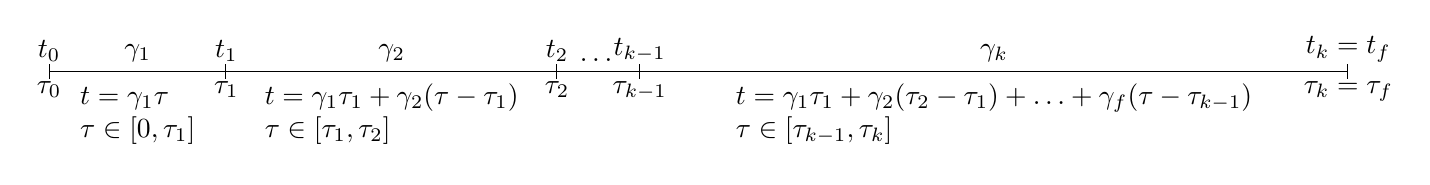
\begin{tikzpicture}[scale=1.5, domain=0:4, samples=200]
	    \draw [|-|](0,0) node[above] {$t_0$} node[below] {$\tau_0$} -- (1.5,0) node[midway, above] {$\gamma_1$} node[midway, below] {\begin{tabular}{l}
	    	$t = \gamma_1\tau$ \\
	    	$\tau\in[0, \tau_1]$
	    	\end{tabular}};
	    \draw [-|](1.5,0) node[above] {$t_1$} node[below] {$\tau_1$} -- (4.3,0) node[midway, above] {$\gamma_2$} node[midway, below] {\begin{tabular}{l}
	    	$t = \gamma_1\tau_1+\gamma_2(\tau-\tau_1)$ \\
	    	$\tau\in[\tau_1, \tau_2]$
	    	\end{tabular}};
	    \draw [-|](4.3,0) node[above] {$t_2$} node[below] {$\tau_2$} -- (5,0) node[midway,above] {\dots};
	    \draw [-|](5,0) node[above] {$t_{k-1}$} node[below] {$\tau_{k-1}$} -- (11,0) node[midway, above] {$\gamma_k$} node[midway, below] {\begin{tabular}{l}
	    	$t = \gamma_1\tau_1+\gamma_2(\tau_2-\tau_1)+\dots+\gamma_f(\tau-\tau_{k-1})$ \\
	    	$\tau\in[\tau_{k-1}, \tau_k]$
	    	\end{tabular}} node[above] {$t_k = t_f$} node[below] {$\tau_k = \tau_f$};
	\end{tikzpicture}
	\caption{Mehrere miteinander gekoppelte Zeitintervalle, die sich zu einem Gesamtintervall $[\tau_0, \tau_f]$ zusammensetzen.}
	\label{fig:Zeittransformation}
\end{figure}
Für die einzelnen Teilintervalle gelten dabei die dargestellten Zeittransformationen, sodass für das $j$-te Teilintervall
\begin{equation}
	\frac{\partial t}{\partial\tau} = \gamma_j \,, \quad\textrm{mit}\, j=1,2,...,k
\end{equation}
und damit 
\begin{equation}
\ve{z}_j'(\tau) = 
\gamma_j
\begin{bmatrix}
\ve{f}(\xoftau,\uoftau,\tau) \\
-\frac{\partial H}{\partial \ve{x}}
\end{bmatrix} 
\end{equation} 
gilt. Auch hier lassen sich die festen Intervallgrenzen ohne Einschränkung der Allgemeinheit zu
\begin{equation}
	\tau_0 = 0\,, \quad\tau_j = j\,, \quad\textrm{mit}\, j=1,2,...,k
\end{equation}
wählen, sodass für die freien Intervallgrenzen 
\begin{align}
t_0 &= \tau_0 = 0\\
t_1 &= \gamma_1 \\
t_2 &= \gamma_1+\gamma_2 \\
&\vdots\\
t_f = t_k &= \gamma_1+\gamma_2+\dots+\gamma_k
\end{align}
gilt. Mithilfe dieser Erweiterung lassen sich beliebig viele Intervalle fester Intervallgrenzen auf Intervalle freier Grenzen transformieren. Eine Anwendung derartig verknüpfter Zeittransformationen kann nützlich sein, wenn mehrere \gls{OP}, die jeweils für ein Teilintervall gelten, betrachtet werden und die Übergangsstellen $t_j$ frei und damit Teil der Optimierung sein sollen. Dann lassen sich die entsprechenden Teilintervalle mit festen Grenzen definieren und wie dargestellt mithilfe der Transformationsvorschriften auf die gesuchten, freien Intervallgrenzen abbilden.
\section{Variationsprobleme mit internen Gleichungsnebenbedingungen}\label{sec:InterneGNB}
Es kann durchaus von Interesse sein, neben den Randbedingungen an den Zeitpunkten $t_0$ und $t_f$ zusätzliche interne Randbedingungen der Form
\begin{equation}
	\tilde{\mathbf{g}}(\xoftone,t_1) = 0 \label{eq:NBt1}
\end{equation} zu formulieren, die die optimalen Trajektorien erfüllen sollen, wenn das dynamische System beispielsweise einen bestimmten Zustand zu einem gewissen Zeitpunkt $t_1$ erreichen soll \cite{Papageorgiou.2012}. Dazu wird auch in diesem Fall das Gütefunktional in Gleichung \eqref{eq:J_var_sys} analog zur Betrachtung allgemeiner Endbedingungen erweitert und lautet 
\begin{equation}
\begin{split}
J(\ve{x},\dx,\ve{u},t,t_f,t_1) &= \underbrace{\Vofxoftf + \ve{\nu}^T\mathbf{g}(\xoftf,t_f) + \Vofxoftone + \tilde{\ve{\nu}}^T\tilde{\mathbf{g}}(\xoftone,t_1)}_{\Vofxoftoftonefallgemein} + \dots \\
\dots&+\int_{t_0}^{t_f}l(\ve{x},\ve{u},t) + \ve{\lambda}^T(\ve{f}(\ve{x},\ve{u},t) - \dx)\dtint{t}\,. \label{eq:J_var_sys_t1}
\end{split}
\end{equation}
Allgemein können die Systemzustände und die adjungierten Zustände an der Stelle $t_1$ unstetig sein \cite{Gerdts.2010}, weshalb es zweckmäßig ist, die Zeitpunkte $t_1^-$ und $t_1^+$ als die Zeitpunkte unmittelbar vor und nach der Sprungstelle $t_1$ zu definieren. Der Zeitpunkt $t_1$ kann wie bereits der Endzeitpunkt $t_f$ entweder festgelegt oder frei sein. An der Übergangsstelle $t_1$ ergeben sich die Transversalitätsbedingungen \cite{Gerdts.2010}
\begin{align}
\Big(\frac{\partial \tilde{V}}{\partial \xoftone} + (\frac{\partial \tilde{\mathbf{g}}}{\partial \xoftone})^T\tilde{\ve{\nu}} - \lambdaoftone\Big)_{|t_1=t_1^-} &= 0 \label{eq:Sprungbedingung1}\\
\Big(\frac{\partial \tilde{V}}{\partial \xoftone} + (\frac{\partial \tilde{\mathbf{g}}}{\partial \xoftone})^T\tilde{\ve{\nu}} + \lambdaoftone\Big)_{|t_1=t_1^+} &= 0 \label{eq:Sprungbedingung2}\\
H(\ve{x},\ve{u},\ve{\lambda},t)_{|t=t_1^-} - H(\ve{x},\ve{u},\ve{\lambda},t)_{|t=t_1^+} + \Big(\frac{\partial \tilde{V}}{\partial t}+(\frac{\partial \tilde{\mathbf{g}}}{\partial t})^T\tilde{\ve{\nu}}\Big)_{|t=t_1}&= 0\,,\quad \textrm{falls, $t_1$ frei ist.}\label{eq:Transversalität_t1}
\end{align}
Zwei Spezialfälle spielen für die Anwendung der zusätzlichen Transveralitätsbedingungen eine besondere Rolle und werden an dieser Stelle nochmal hervorgehoben. 
\begin{enumerate}
	\item Wie bereits erwähnt, können die Systemzustände \xoft\,an der Übergangsstelle $t_1$ allgemein unstetig sein und einen Sprung aufweisen. Bei der Behandlung dynamischer Systeme, die ein reales System repräsentieren, ist ein derartiges sprunghaftes Verhalten oftmals unerwünscht, da es auf der einen Seite nicht realisierbar ist und auf der anderen Seite unkomfortable Trajektorien bedeutet. Daher sind häufig solche Lösungen von Interesse, bei denen zumindest die Systemzustände \xoft\,in $t_1$ stetig sind, also 
	\begin{equation}
		\xoftoneminus = \xoftoneplus \label{eq:Stetigkeit_t1}
	\end{equation}
	gilt. Damit lassen sich die Randbedingungen \eqref{eq:Sprungbedingung1} und \eqref{eq:Sprungbedingung2} zur sogenannten \textit{ersten Weierstrass-Erdmannschen-Eckenbedingung} zusammenfassen \cite{Gerdts.2010}:
	\begin{equation}
		2\Big(\frac{\partial \tilde{V}}{\partial \xoftone} + (\frac{\partial \tilde{\mathbf{g}}}{\partial \xoftone})^T\tilde{\ve{\nu}}\Big) - \lambdaoftoneminus + \lambdaoftoneplus = 0\,. \label{eq:WeierstrassErdmann1}
	\end{equation}
	Die adjungierten Zustände \lambdaoft\,können dabei in $t_1$ weiterhin sprunghaft sein, was allderings nicht problematisch ist, da sie keine physikalischen Größen darstellen.
	\item Der zweite Sonderfall ergibt sich, wenn $t_1$ zwar frei ist, aber die Nebenbedingung \eqref{eq:NBt1} und die zusätzlichen Kosten \Vofxoftone\,nicht explizit von $t_1$ abhängen, also $\tilde{\mathbf{g}}(\xoftone) = 0$ und $\tilde{V}(\ve{x}(t_1))$ gilt. Gleichung \eqref{eq:Transversalität_t1} wird dann zur \textit{zweiten Weierstrass-Erdmannschen-Eckenbedingung}, aus der die Stetigkeit der Hamilton-Funktion in $t_1$ folgt \cite{Gerdts.2010}:
	\begin{equation}
	H(\ve{x},\ve{u},\ve{\lambda},t)_{|t=t_1^-} = H(\ve{x},\ve{u},\ve{\lambda},t)_{|t=t_1^+}\,. \label{eq:WeierstrassErdmann2}
	\end{equation}
\end{enumerate}
\section{Diskontinuierliche Systemdynamik}\label{sec:Diskontinuität}
Die Verwendung von diskontinuierlicher Systemdynamik liefert eine überaus nützliche Methode zur Betrachtung unterschiedlicher Zustandsgleichungen in einem \gls{OP}. Mithilfe dieser Methode können verschiedene, in unterschiedlichen Bereichen geltende Systembeschreibungen in einem \gls{OP} verwendet werden, sodass sich einzelne Szenarien miteinander zu einem Gesamtszenario kombinieren lassen. Diese Methode findet bspw. in dem in Abschnitt \ref{subsec:Optimalitätsprinzip} skizzierten Abbiegeszenario Verwendung. Die drei Teilszenarien Gerade, Kurve und Gerade lassen sich mithilfe von Übergangsbedingungen verknüpfen und in den einzelnen Teilbereichen gilt jeweils die für das entsprechende Teilszenario formulierte Systemdynamik. Die Systemdynamik des Gesamtszenarios lässt sich aus $k$ Teilszenarien wie folgt zusammensetzen \cite{Papageorgiou.2012}:
\begin{equation}
\dx = \ve{F}(\ve{x},\ve{u},t) = \left\{\begin{matrix}
\ve{f}_1(\ve{x},\ve{u},t)\,, & \mathrm{falls} & \begin{matrix}\tilde{\mathbf{g}}_i(\ve{x},t) \leq 0 \quad\forall\, i = 1,2,...,k-1\end{matrix}\\
\ve{f}_2(\ve{x},\ve{u},t)\,, & \mathrm{falls} & \begin{matrix}
\tilde{\mathbf{g}}_{\hat{i}}(\ve{x},t) > 0 \quad\forall\, \hat{i} = 1 \quad\textrm{und} \\ \tilde{\mathbf{g}}_i(\ve{x},t) \leq 0 \quad\forall\, i = 2,...,k-1
\end{matrix}\\
\vdots & & \\
\ve{f}_j(\ve{x},\ve{u},t)\,, & \mathrm{falls} & \begin{matrix}
\tilde{\mathbf{g}}_{\hat{i}}(\ve{x},t) > 0 \quad\forall \, \hat{i} = 1,2,...,j-1 \quad\textrm{und} \\ \tilde{\mathbf{g}}_i(\ve{x},t) \leq 0 \quad\forall\, i = j,...,k-1
\end{matrix}\\
\vdots & & \\
\ve{f}_k(\ve{x},\ve{u},t)\,, & \mathrm{falls} & \begin{matrix}\tilde{\mathbf{g}}_{\hat{i}}(\ve{x},t) > 0 \quad\forall\, \hat{i} = 1,2,...,k-1
\end{matrix}
\end{matrix}\right. \label{eq:Diskontinuität}
\end{equation}
Die Gleichungen $\tilde{\mathbf{g}}_i(\xofti,t_i) = 0$ nehmen dabei die Funktion der $k-1$ Übergangsbedingungen zu den Zeitpunkten $t_i$ ein, zu denen von der einen Systemdynamik zur nächsten gewechselt wird und werden analog zu den Ausführungen in Abschnitt \ref{sec:InterneGNB} wie interne \gls{GNB} behandelt. Für jeden der Übergangspunkte gelten die Transversalitätsbedingungen \eqref{eq:Sprungbedingung1} - \eqref{eq:Transversalität_t1} bzw. \eqref{eq:Stetigkeit_t1} - \eqref{eq:WeierstrassErdmann2}, wobei insbesondere bei der zweiten Weierstrass-Erdmannschen-Eckenbedingung darauf geachtet werden muss, dass sich auch die Hamilton-Funktion aufgrund der wechselnden Systemdynamik gemäß
\begin{equation}
	H_j(\ve{x},\ve{u},\ve{\lambda},t) = l(\ve{x},\ve{u},t) + \ve{\lambda}^T\ve{f}_j(\ve{x},\ve{u},t) \label{eq:Hamilton_j}
\end{equation} 
verändert. Damit lautet die zweite Weierstrass-Erdmannsche-Eckenbedingung in Gleichung \eqref{eq:WeierstrassErdmann2} an der Übergangsstelle $t_i$
\begin{equation}
H_i(\ve{x},\ve{u},\ve{\lambda},t)_{|t=t_i^-} = H_{i+1}(\ve{x},\ve{u},\ve{\lambda},t)_{|t=t_i^+}\,. \label{eq:WeierstrassErdmann2_j}
\end{equation}

Die in diesem Kapitel beschriebenen Methoden liefern das Handwerkszeug, um dynamische \gls{OP} mithilfe der Variationsrechnung zu lösen und die Problemstellung so zu formulieren, dass komplexe Fahrszenarien durch geschickte Kombination mehrerer Teilszenarien vereinfacht und analytisch gelöst werden können. Das Optimalitätsprinzip nach Bellmann (siehe Abschnitt \ref{subsec:Optimalitätsprinzip}) liefert die Grundlage dafür, dass mehrere Teilprobleme die optimale Lösung für ein Gesamtproblem ergeben. Mithilfe von Zeittransformationen und unter Verwendung diskontinuierlicher Systemdynamik (Abschnitte \ref{sec:Zeittransformation} und \ref{sec:Diskontinuität}) lassen sich auf frei wählbaren Zeitintervallen beliebig viele Teilsysteme unterschiedlicher Systemdynamik miteinander kombinieren, wobei sich mithilfe der Nebenbedingungen an den internen Übergangspunkten (siehe Abschnitt \ref{sec:InterneGNB}) Stetigkeit der Systemzustände erzielen lassen, während weiterhin die Optimalität der Lösung gewährleistet ist.
\section{Numerische Lösungsverfahren}\label{sec:Lösungsverfahren}
Dieser Abschnitt dient der Übersicht über unterschiedliche numerische Lösungsverfahren für dynamische \gls{OP}. Dazu sollen einige Verfahren erläutert und hinsichtlich ihrer Vor- und Nachteile miteinander verglichen werden. Zunächst wird der Unterschied zwischen \textit{indirekten} und \textit{direkten} Lösungsverfahren erklärt und anschließend jeweils verschiedene Verfahren der beiden Verfahrensklassen vorgestellt.
\subsection{Indirekte Lösungsverfahren}\label{subsec:Indirekt}
Bei den indirekten Lösungsverfahren wird mithilfe der Optimalitätsbedingungen \eqref{eq:Zustandsdgl}-\eqref{eq:Steuerungsgleichung} und den Randbedingungen \eqref{eq:Anfangswerte}-\eqref{eq:Transversalitaet} das entstehende Randwertproblem gelöst \cite{Papageorgiou.2012} - die indirekten Lösungsverfahren basieren also auf der Anwendung der Variationsrechnung. Die Lösung kann dabei entweder analytisch oder mithilfe numerisch ermittelt werden \cite{Gerdts.2010}. Im Gegensatz zu den direkten Lösungsverfahren wird das dynamische \gls{OP} bzw. Optimalsteuerungsproblem bei indirekten Verfahren nicht zunächst diskretisiert, sondern es werden direkt die Optimalitätsbedingungen für das entsprechende \gls{OP} hergeleitet, weshalb bei den direkten Verfahren auch von einer ``\textit{first optimize, then discretize''}-Strategie gesprochen wird \cite{Papageorgiou.2012} - dies trifft insbesondere auf indirekte Diskretisierungsverfahren zu (siehe Abschnitt \ref{subsubsec:Diskretisierungsverfahren_indirekt}). Dadurch, dass das dynamische \gls{OP} bei indirekten Verfahren nicht zuerst in ein statisches Ersatzproblem umgewandelt, sondern stattdessen mithilfe der Variationsrechnung ein Randwertproblem gelöst wird, besitzen sie den großen Vorteil, dass sie zum einen sehr genaue Lösungen liefern und zum anderen Informationen über die Struktur der optimalen Lösung liefern \cite{KnutGraichen.2012}. Selbst wenn das Randwertproblem nicht analytisch gelöst werden kann, so lassen sich trotzdem aus der Lösung der kanonischen \gls{DGL} Erkenntnisse gewinnen, die vor allem für die Interpretation der optimalen Trajektorien sehr wertvoll sein können. Ein weiterer Vorteil indirekter Lösungsverfahren ist, dass die adjungierten Zustände zur Sensitivitätsanalyse des Gütefunktionals gegenüber Änderungen der Anfangszustände \xzero\,verwendet werden können \cite{KnutGraichen.2012}. Indirekte Lösungsverfahren haben den Nachteil, dass die Lösbarkeit eines dynamischen \gls{OP} mittels eines indirekten Verfahrens von der Struktur des \gls{OP} selbst abhängt. Das bedeutet, dass die Herleitung der kanonischen \gls{DGL} und die Tatsache, ob überhaupt eine Lösung angegeben werden kann, sowie die Lösbarkeit des resultierenden Randwertproblems von der Problemstellung selbst abhängen. Die Optimalitätsbedingungen und die Randbedingungen aufzustellen kann für komplizierte Systeme sehr aufwändig sein \cite{Papageorgiou.2012}. Außerdem benötigen indirekte Lösungsverfahren häufig Startschätzungen für die adjungierten Zustände. Die Schätzung dieser Initialwerte beeinflusst die Qualität der Lösung bzw., ob das Verfahren überhaupt konvergiert, sodass der Konvergenzbereich indirekter Verfahren oftmals nicht sehr groß ist \cite{Papageorgiou.2012}. Nachfolgend werden einige indirekte Lösungsverfahren vorgestellt und hinsichtlich des \gls{AD}-Planungsproblems diskutiert. 
\subsubsection{Indirekte Diskretisierungsverfahren}\label{subsubsec:Diskretisierungsverfahren_indirekt}
Der ``\textit{first optimize, then discretize''}-Ansatz für indirekte Lösungsverfahren trifft vor allem auf indirekte Diskretisierungverfahren zu. Entsprechend der Ausführungen in Abschnitt \ref{sec:dynamischeOpt} werden die \gls{DGL} \eqref{eq:Sysdyn_z} über den Ansatz der Variationsrechnung hergeleitet. Gemeinsam mit den Randbedingungen \eqref{eq:Anfangswerte}-\eqref{eq:Transversalitaet} ergibt sich ein \gls{ZPR}, welches auf dem Gesamtintervall $[t_0, t_f]$ an $N+1$ Stützstellen diskretisiert wird \cite{KnutGraichen.2012} - das Problem wird also zuerst optimiert und anschließend diskretisiert. Dieses Randwertproblem wird mithilfe eines numerischen Integrationsverfahrens, wie zum Beispiel dem Verfahren von Heun, bei dem ein Trapez zur Approximation des Integrals verwendet wird (siehe auch \cite{Adamy.2009} für Informationen zu weiteren Verfahren), unter Berücksichtigung der Randbedingungen gelöst \cite{KnutGraichen.2012}. Da die zu lösenden \gls{DGL} bei der numerischen Integration durch Differenzenquotienten ersetzt werden, werden Diskretisierungsverfahren auch als Differenzenverfahren bezeichnet \cite{Ascher.1995c5}.
\begin{multicols}{2}
Vorteile:
	\begin{itemize}
		\item Numerische Robustheit aufgrund simultaner Berücksichtigung der kanonischen \gls{DGL} und Randbedingungen \cite{KnutGraichen.2012}
		\item Erhöhung der Genauigkeit durch Steigerung der Anzahl der Diskretisierungsstellen \cite{KnutGraichen.2012}
		\item Durch Anwendung von Runge-Kutta-Verfahren mit höherer Verfahrensordnung, lässt sich die Genauigkeit der Integralapproximation verbessern \cite{Ascher.1995c5}
	\end{itemize}
	
	\columnbreak
	
Nachteile:
	\begin{itemize}
		\item Steuergröße $\ve{u}$ muss explizit nach $\ve{x}$ und $\ve{\lambda}$ auflösbar sein \cite{KnutGraichen.2012}\vspace{\fill}
		\item Gute Initialschätzung für \lambdaoftzero\,notwendig \cite{KnutGraichen.2012}\vspace{\fill}
		\item Größere Anzahl an Diskretisierungsstellen steigert den Rechenaufwand \cite{KnutGraichen.2012}\vspace{\fill}
	\end{itemize}
\end{multicols}

\subsubsection{Indirekte Schießverfahren}\label{subsubsec:Schießverfahren_indirekt}
Indirekte Schießverfahren gehen ebenfalls von den \gls{DGL} in Gleichung \eqref{eq:Sysdyn_z} aus. Im Gegensatz zum indirekten Diskretisierungsverfahren wird beim Einfachschießverfahren die Lösung ausgehend von einem Anfangswertproblem berechnet \cite{Papageorgiou.2012}, anstelle des \gls{ZPR}. Dazu wird aus den Anfangswerten \xzero\,und einer Initialschätzung $\ve{\lambda}_0^{(0)}$ für die adjungierten Zustände der Startvektor $\ve{z}_0 = \begin{bmatrix}\xzero^T & \ve{\lambda}_0^{(0)T}\end{bmatrix}^T$ gebildet. Von diesem Startvektor ausgehend werden die \gls{DGL} anschließend bis $t_f$ numerisch vorwärts integriert. Nach Abschluss der Integration erhält man ein Ergebnis für $\lambdaoftf^{(0)}$, welches mit den Randbedingungen \eqref{eq:Lambdaend} verglichen wird. Die Abweichungen in den Randbedingungen lassen sich durch den Fehlervektor $\ve{e}^{(l)} = \lambdaoftf - \ve{\lambda}(t_f)^{(l)}$ ausdrücken, der durch Verbesserung der Startschätzung $\ve{\lambda}_0^{(l)}$ so lange verringert wird, bis eine gewünschte Fehlertoleranz nicht mehr überschritten wird und damit das Ergebnis einer vorgegebenen Güte entspricht \cite{Papageorgiou.2012}. Der hochgestellte Index $(l)$ gibt dabei die $l$-te Iteration der Integration an. Der Startwert $\ve{\lambda}_0^{(l+1)}$ der nächsten Iteration kann zum Beispiel durch Anwendung des Newton-Verfahrens aktualisiert werden \cite{Papageorgiou.2012}.
Auch freie Endzeiten $t_f$ können beim Schießverfahren berücksichtigt werden. Dazu wird analog zu den adjungierten Anfangszuständen eine Initialschätzung $t_f^{0}$ vorgegeben und der Fehlervektor um die Transversalitätsbedingung für freie Endzeit \eqref{eq:Transversalitaet} erweitert \cite{Papageorgiou.2012}.
\begin{multicols}{2}
	Vorteile:
	\begin{itemize}
		\item ``Einfache'' Methode mit geringem Implementierungsaufwand \cite{Ascher.1995c4}\vspace{\fill}
		\item Mehrfachschießverfahren bietet die Möglichkeit der Parallelisierung \cite{Betts.1998}\vspace{\fill}
		\item[\vspace{\fill}]
	\end{itemize}
	
	\columnbreak
	
	Nachteile:
	\begin{itemize}
		\item Instabile Anfangswertprobleme führen dazu, dass das Einfachschießverfahren instabil wird \cite{Ascher.1995c4}, wobei gezeigt werden kann, dass die kanonischen \gls{DGL} im linearen Fall immer an der imaginär Achse gespiegelte Eigenwerte und damit instabile Eigenmoden besitzen, selbst wenn das lineare System stabil ist \cite{KnutGraichen.2012}. 
		\item Empfindlichkeit gegenüber schlechten Startschätzungen für $\ve{\lambda}_0^{(0)}$, sodass unter Umständen keine Lösung auf dem gesamten Integrationsintervall $[t_0, t_f]$ gefunden werden kann \cite{Ascher.1995c4}.
		\item Eingeschränkte Anwendbarkeit für kleine Probleme aufgrund der numerischen Berechnungsschwierigkeiten \cite{Papageorgiou.2012}.
	\end{itemize}
\end{multicols}

Dem Problem der numerischen Stabilität und dem Umstand, dass das Anfangswertproblem ggf. nicht bis zur rechten Intervallgrenze integriert werden kann, kann mit dem Mehrfachschießverfahren begegnet werden. Ähnlich zum Diskretisierungsverfahren wird das Integrationsintervall beim Mehrfachschießverfahren ebenfalls in $N$ Subintervalle aufgeteilt. Auf jedem der Subintervalle wird das Anfangswertproblem \eqref{eq:Sysdyn_z} mit $\ve{z}(t_j) = \begin{bmatrix}\ve{x}_j^T & \ve{\lambda}_j^T\end{bmatrix}^T$ und $t\in[t_j, t_{j+1}),\,j = 0,1,...,N-1$ mittels Einfachschießverfahren gelöst \cite{Gerdts.2010}. Damit die Lösung der einzelnen Anfangswertprobleme auf den Subintervallen tatsächlich eine Lösung des ursprünglichen \gls{ZPR} ist, müssen neben den Randbedingungen, die sich über die Formulierung der Optimalitätsbedingungen ergeben, noch die Stetigkeitsbedingungen \begin{equation*}
	\begin{bmatrix}
	\ve{z}_0(t_1,\begin{bmatrix}\ve{x}_0^T & \ve{\lambda}_0^T\end{bmatrix}^T) - \begin{bmatrix}\ve{x}_1^T & \ve{\lambda}_1^T\end{bmatrix}^T \\
	\ve{z}_1(t_2,\begin{bmatrix}\ve{x}_1^T & \ve{\lambda}_1^T\end{bmatrix}^T) - \begin{bmatrix}\ve{x}_2^T & \ve{\lambda}_2^T\end{bmatrix}^T \\
	\vdots \\
	\ve{z}_{N-2}(t_{N-1},\begin{bmatrix}\ve{x}_{N-2}^T & \ve{\lambda}_{N-2}^T\end{bmatrix}^T) - \begin{bmatrix}\ve{x}_{N-1}^T & \ve{\lambda}_{N-1}^T\end{bmatrix}^T
	\end{bmatrix} = \ve{0}
\end{equation*}
zwischen den einzelnen Subintervallen erfüllt sein \cite{Gerdts.2010}. Das Ergebnis des Anfangswertproblems am Intervallende des $j$-ten Subintervalls muss also dem Anfangswert der Lösung auf dem $j+1$-ten Intervall entsprechen. Mit dieser Erweiterung auf Mehrfachschießverfahren lässt sich die Robustheit der numerischen Integration auf Kosten des Rechenaufwands steigern, da der Rechenaufwand durch die Intervallunterteilung ansteigt \cite{Betts.1998}.
\subsubsection{Indirekte Kollokationsverfahren}\label{subsubsec:Kollokationsverfahren_indirekt}
\subsubsection{Indirekte Gradientenverfahren}\label{subsubsec:Gradientenverfahren_indirekt}
\subsection{Direkte Lösungsverfahren}\label{subsec:Direkt}
Unabhängig davon, wie genau ein allgemeines dynamisches \gls{OP} (\eqref{eq:J_dyn}- \eqref{eq:UNB}) durch ein bestimmtes direktes Lösungsverfahren gelöst wird, haben die direkten Verfahren alle eines gemeinsam: Das dynamische \gls{OP} wird mittels Diskretisierung in ein statisches Ersatzproblem überführt, wobei die Steuertrajektorie \uoft\,an $N$ Stützstellen diskretisiert wird \cite{KnutGraichen.2012}. Dadurch wird aus dem dynamischen \gls{OP} ein endlich dimensionales statisches \gls{OP}, welches in der allgemeinen Form \eqref{eq:J_statisch}-\eqref{eq:UNB_statisch} geschrieben werden kann und bezüglich der Optimierungsvariablen $\ve{u}_i$ mit $i=0,1,...N-1$ optimiert wird. Aufgrund dieser Vorgehensweise werden direkte Verfahren auch als ``\textit{first discretize, then optimize''}-Strategie bezeichnet \cite{Papageorgiou.2012}. Ein wesentlicher Unterschied zwischen direkten und indirekten Verfahren, liegt darin, dass die Optimalitätsbedingungen aus der Variationsrechnung bei direkten Verfahren nicht explizit berücksichtigt werden müssen \cite{Rathgeber.2016}. Diese Eigenschaft macht direkte Lösungsverfahren besonders attraktiv für komplizierte Anwendungen \cite{Betts.1998}. Ungeachtet der Komplexität der Lösung lässt sich das dynamische \gls{OP} mithilfe der Diskretisierung immer auf ein statisches Ersatzproblem zurückführen, wodurch sich direkte Methoden robust anwenden lassen und sich vielseitige Anwendungsbereiche ergeben \cite{Betts.1998}. Weitere Vorteile direkter Lösungsverfahren liegen zum einen darin, dass sich aufgrund der Diskretisierung der Trajektorien Zustandsbeschränkungen sowohl in Form von \gls{GNB} als auch \gls{UNB} leicht berücksichtigen lassen \cite{KnutGraichen.2012}. Zum anderen hängt die Qualität der Lösung nicht von Startschätzungen für die adjungierten Zustände ab, die bei indirekten Verfahren angegeben werden müssen, weshalb sich oftmals größere Konvergenzbereiche für direkte Verfahren ergeben \cite{KnutGraichen.2012}. Ein Nachteil von direkten Lösungsverfahren liegt darin, dass die Optimierungsvariablen das optimale Systemverhalten nur an den diskretisierten Stützstellen wiedergeben, weshalb direkte Verfahren ggf. nicht die gewünschte Lösungsgenauigkeit erreichen \cite{Papageorgiou.2012}. Außerdem liefert die Lösung keine Erkenntnisse über die analytische Struktur der optimalen Verläufe. Mithilfe einer höherfrequenten Diskretisierung in engeren Schritten lässt sich die Übereinstimmung der direkten Lösung mit dem analytischen Verlauf der optimalen Lösung und damit die Qualität der direkten Lösung verbessern, allerdings bedeutet dies eine Zunahme der Dimension des Problems. Gerade Systeme hoher Ordnung können auf diese Weise schnell in eine Größenordnung anwachsen, dass sie sich nicht mehr oder nur sehr langsam lösen lassen, abhängig davon wie viel Rechenleistung und Speicherkapazität zur Verfügung stehen \cite{Papageorgiou.2012}. Dies war lange Zeit ein maßgeblich beschränkender Faktor in der Anwendung direkter Lösungsverfahren, der mittlerweile aufgrund des heutigen Fortschritts bei der Entwicklung leistungsfähiger Rechner immer mehr in den Hintergrund gerückt ist \cite{Papageorgiou.2012}. Im Folgenden werden drei Arten von direkten Lösungsverfahren vorgestellt, die einen Großteil der Klasse direkter Lösungsverfahren widerspiegeln \cite{Papageorgiou.2012}. 
\subsubsection{Direkte Diskretisierungsverfahren}\label{subsubsec:Diskretisierungsverfahren_direkt}
\subsubsection{Direkte Schießverfahren}\label{subsubsec:Schießverfahren_direkt}
\subsubsection{Direkte Kollokationsverfahren}\label{subsubsec:Kollokationsverfahren_direkt}

